\chapter{Vademecum d'électricité}
\section{Notions fondamentales}
\subsection{Schémas}
Tout schéma possède un sens de lecture, de l'entrée vers la sortie. La \textit{charge}
est le composant connecté en aval d'un montage. Lorsque celle-ci est retirée
le montage fonctionne à vide. La \textit{source} est exactement l'opposé,
c'est à dire le composant connecté en amont d'un montage.

\subsection{Les éléments : dipôles et quadripôles}
\begin{wrapfigure}[4]{r}{3cm}
	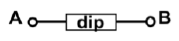
\includegraphics[scale=0.5]{img/image1.png}
	\captionof{figure}{Dipôle}
\end{wrapfigure}
Tout élément possède un certain nombre de \textit{bornes} (caractérisée par un potentiel électrique et une valeur de courant\footnote{Lorsque $I$ est identique aux deux bornes, on peut les associer et parler de \textbf{port} ou \textbf{accès}. Le dipôle est par définition un accès.}) qui servent à établir des connexions, un dipôle est simplement un élément en possédant deux.

\subsubsection{Nœud, branche et maille}
\begin{wrapfigure}[9]{l}{6cm}
	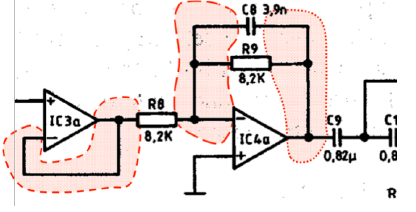
\includegraphics[scale=0.5]{img/image2.png}
	\captionof{figure}{Nœud}
\end{wrapfigure}
On connecte les éléments par des bornes : lorsqu'on connecte plusieurs éléments ensemble on forme un noeud, qui est par définition équipotentiel.\\
\textbf{Attention !} Le noeuds couvre l'ensemble de la connexion et pas seulement le point de contact des fils.\\

Tout dipole ou assemblage de dipole en série constitue une \textbf{branche} est l'ensemble de ces branches constituant un parcours fermé constitue une \textbf{maille}.

\subsubsection{Composants en série/en parallèle}
Les deux règles à retenir sont :
\begin{enumerate}
	\item Deux composants sont connectés en série s'ils sont parcourus par le même
	      courant.
	\item Deux composants sont connectés en parallèle s'ils sont soumis à la même
	      différence de potentiel.
\end{enumerate}

\subsection{Courant}
Le \textbf{courant} est un déplacement d'ensemble de charges électriques dans un conducteur.\\
Notons qu'un courant est généralement constitué d'électrons mais que ce-dernier peut également être constitué d'électrolytes ou de semi-conducteurs.

\subsubsection{Intensité = valeur du courant électrique}
L'\textbf{intensité} est le débit de charge électrique :
\begin{equation}
	i(t) = \frac{dq(t)}{dt}
\end{equation}

\subsubsection{Mesure du courant électrique}
Il faut insérer un ampèremètre \textbf{en série} avec le fil dans lequel on désire mesurer le courant.

\subsubsection{Représentation du courant : sens conventionnel}
\begin{wrapfigure}[5]{l}{3.5cm}
	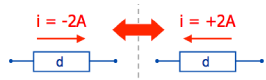
\includegraphics[scale=0.5]{img/image3.png}
	\captionof{figure}{Inversion du sens}
\end{wrapfigure}
Il s'agit d'une flèche qui pointe dans la direction de charge qui seraient positives : il s'agit du sens de courant conventionnel qui est toujours représenté dans les schéma.\\
Si le courant était négatif, on peut le rendre positif en inversant le sens de la flèche.

\subsubsection{Circulation du courant en boucle fermée}
"Un chemin de retour" doit toujours exister. Branche interrompue : courant nul.

\subsection{Tension(s)}
\subsubsection{La tension : un terme ambigu}
C'est un terme ambigu car il peut être trois chose distinctes : la force électromotrice, le potentiel d'un noeud ou la d.d.p.

\subsubsection{DDP et potentiel}
\subsubsection{Différence de potentiel}
C'est ce qui se mesure en pratique (à l'aide d'un multimètre, sur un dipôle), il s'agit de la différence de potentiel entre deux bornes.

\subsubsection{Potentiel électrique (première approche)}
C'est une notion purement théorique qui se résume à dire que le potentiel électrique en un point est l'énergie à dépenser pour amener une charge unitaire depuis un point ou le potentiel est nul (à l'infini).

\subsubsection{Convention et signes}
\subsubsection{Convention concernant le sens de la différence de potentiel}
La ddp étant une soustraction, il faut définir le sens de celle ci.
Lorsque la flèche va de $B$ vers $A$ (convention) :
\begin{equation}
	V = V_A - V_B
\end{equation}
Ceci découle de cette opération "soustraction", la pointe de la flèche pointera vers le potentiel le plus haut.

\subsubsection{Interprétation des notions de potentiel et de masse}
\subsubsection{Potentiel et masse = notion théorique}
Plus utile que le potentiel, on utilise la masse:\\
\prop{La masse est le noeud dont le potentiel, par convention, est nul : $V_{masse} = 0V$}\ \\

C'est un choix arbitraire, une convention qui servira de référence.
Si on connait toutes les ddp, il faut un "repère" sans quoi on ne pourra jamais connaître les potentiels des noeuds (qui est "défini à une constante près").

\subsubsection{Présence/absence de masse}
On n'a pas besoin de masse pour résoudre un circuit sur papier.\\
\prop{Si l'on ne s'intéresse qu'aux ddps, il n'est pas nécessaire de définir une masse}\ \\

\subsubsection{Potentiel représenté comme une ddp}
\prop{La ddp entre un noeud A quelconque et la masse est numériquement égale au potentiel de ce noeud A}\ \\

\subsubsection{Tension différentielle}
Souvent, en présence de masse, on calcule la ddp par rapport avec celle-ci. Si la masse n'est pas présente on parlera de \textbf{tension différentielle} pour bien différencier les deux.

\subsubsection{Terre = protection}
\begin{wrapfigure}[5]{r}{2.5cm}
	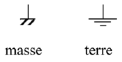
\includegraphics[scale=0.5]{img/image4.png}
	\captionof{figure}{Symboles}
\end{wrapfigure}
Il ne faut pas confondre les deux, la terre est une notion pratique relative à la sécurité des personnes et des équipements.

\subsection{Puissane instantanée, conventions et passivité}
\subsubsection{Dipôles actifs et passif - définition intuitive.}
\begin{itemize}
	\item[Passif] : Ne peut qu'absorber l'énergie (résistance, condensateur, ...)
	\item[Actif] : Injecte de l'énergie dans le circuit (source de tension, pile, ...)
\end{itemize}

\subsubsection{Puissance instantanée sur un dipôle}
La puissance électrique est l'énergie fournie ou reçu par unité de temps par un dipôle
\begin{equation}
	p(t) = v(t).i(t)
\end{equation}

\subsection{Conventions récepteurs et générateur}
Dans tout dipôle passif, les flèches courant et tension doivent être de sens opposés : \textbf{convention récepteur}.\\
\begin{wrapfigure}[8]{r}{3cm}
	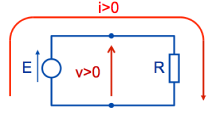
\includegraphics[scale=0.5]{img/image5.png}
	\captionof{figure}{Conv. générateur}
\end{wrapfigure} Dans cette convention, la formule $p(t)$ donne la puissance instantanée absorbée par ce dipôle.

Dans la source par contre, ces deux flèches doivent être dans le même sens. La formule de puissance donnera dans ce cas la puissance instantanée fournie grâce à la \textbf{convention générateur}.Le rôle de la source est de "relever" le potentiel.

\subsection{Critère de passivité}
\begin{equation}
	w(t) = \int_0^\infty p(t)dt \geq 0
\end{equation}
Un dipôle passif ne peut pas délivrer ce qu'il n'a pas reçu, cela ne peut donc pas être négatif. Si c'est le cas, le dispositif sera \textit{actif}.
 


\newpage
\section{Comportement externe : loi et caractéristique d'un dipôle}
\subsection{Dipôle}
\subsubsection{Etat électrique d'un dipôle}
Il s'agit du couple $(I,V)$ de valeurs électriques mesurables sur un dipôle à l'instant $t$.

\subsubsection{Comportement électrique du dipôle}
Les valeurs que prennent $I$ et $V$.

\subsubsection{Loi du dipôle}
C'est la formule exprimant mathématiquement le comportement.
\begin{itemize}
	\item[Source de tension idéale] : $V = E$ : impose une ddp et ce peu importe le courant qui la traverse (ne modifie par le courant).
	\item[Source de courant idéale] : $I = J$ : impose un courant et ce peu impporte la tension (ne modifie pas la tension).
\end{itemize}

\subsubsection{Caractéristique}
La \textbf{caractéristique} est la représentation graphique du \textit{comportement électrique} du dipôle.\footnote{La caractéristique n'apporte aucune info supplémentaire par rapport à la loi.}

\subsection{Charges idéales : trois effets physiques}
\setcounter{subsection}{1}
\subsubsection{Inductance}
La loi de base est que $\phi \propto I$ impliquant :
\begin{equation}
	\phi (t) = LI
\end{equation}
Comme $v(t) = \frac{d\phi}{dt}$ on peut dire que $v(t) = L\frac{di}{dt}$ et $e(t) = -\frac{d\phi}{dt}$ qui est une autre manière d'exprimer la loi de Lenz. On utilisera :
\begin{itemize}
	\item loi de l'inductance : convention récepteur
	\item loi de Lenz : convention générateur
\end{itemize}

\begin{center}
	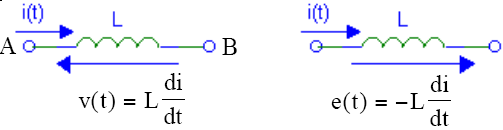
\includegraphics[scale=0.5]{img/image10.png}
	\captionof{figure}{Inductance/Lenz}
\end{center}

La loi courant-tension décrite ci-dessus implique :
\begin{itemize}
	\item si la ddp est \textbf{constante}, le courant croît \textbf{linéairement}
	\item si le courant est \textbf{constant}, la ddp est \textbf{nulle}.
\end{itemize}


\subsubsection{Lois "court terme" et "long terme"}
Dans une self, le courant ne peut pas varier instantanément sinon la ddp serait infinie. Il s'agit de la loi à court terme.\\
Cependant, après un temps infini la ddp doit forcément être nulle sans quoi $I = - \infty$ ce qui est impossible. Il s'agit de la loi à long terme.

\subsubsection{Interprétation physique}
Lorsque 'lon essaye de faire varier le courant dans une self, celle-ci développe une fem qui contre cette variation. La self oppose donc une certaine \textit{inertie} à la variation du courant qui la traverse.\\

Histoire de ne pas l'oublier (et de mettre en avant cet "effet mémoire"), voici la loi courant tension de la self:
\begin{equation}
	i(t) = i(0) + \frac{1}{L}\int_0^t v(t) dt
\end{equation}


\subsection{Capacité}
La loi de base à retenir est que $Q \propto V$.
\begin{equation}
	i(t) = C \frac{dv(t)}{dt}
\end{equation}
où $v$ est la ddp. On dira que
\begin{itemize}
	\item la capa se \textbf{charge} quand la ddp (ou |Q|) \textbf{augmente}
	\item la capa se \textbf{décharge} quand la ddp (ou |Q|) \textbf{diminue}
\end{itemize}


\subsubsection{Interprétation physique}
A cause de la dérivée dans cette expression on remarque, à l'inverse de $R$\footnote{Où courant implique tension}, que c'est la \textit{variation de la ddp} qui implique l'existence d'un courant et inversement.\\
Une capacité n'a pas de caractéristique dans le plan $(I,V)$ car le temps y intervient. Retenons que
\begin{enumerate}
	\item si le courant est constant, la ddp croit linéairement
	\item si la ddp est constante, le courant est nul.
\end{enumerate}

\subsubsection{Lois "court terme" et "long terme"}
On constante que la $ddp$ ne varie pas instantanément sinon $i(t) = \infty$ ce qui est impossible.\\
Après un temps infini, le courant doit forcément être nul sinon la ddp atteindrait une valeur négative infinie ce qui est également impossible.

\subsubsection{Autre interprétation physique}
Pour faire varier la charge, il faut injecter ou retirer des charges à la capacité, ce qui prends un certain temps (pas instantané): il faut qu'un courant circule : on dit que la capacité s'\textbf{oppose/présente une inertie} aux variations de tension

\subsubsection{Charge initiale}
La loi de base exprimée en tension et en courant est 
\begin{equation}
	v(t) = \frac{1}{C} \int_{-\infty}^t i(t) dt
\end{equation}
Ou encore, plus pratiquement (ne pas oublier $v(0)$ qui traduit un "effet de mémoire" :
\begin{equation}
	v(t) = v(0) + \frac{1}{C} \int_0^t i(t) dt
\end{equation}


\subsection{Court-circuit et circuit ouvert}
\subsubsection{Court-circuit}
Il s'agit d'un dipôle imposant une ddp nulle, quelque soit la valeur du courant qui le traverse : $V = 0$.\\ On réalise un court circuit en mettant deux noeuds au même potentiel.
\textbf{Attention !} Ddp nulle n'implique pas que le courant l'est également !

\subsubsection{Circuit ouvert}
Un \textbf{circuit ouvert} est par définition un dipôle traversé par un courant nul, quelque soit la ddp à ses bornes : $I =0$.\\
\textbf{Attention !} Encore une fois, la ddp aux bornes d'un circuit ouvert est à priori \textbf{non} nulle !




\newpage
\section{Circuits équivalents et théorèmes de Thévenin/Norton}
\subsection{Théorèmes de Thévenin/Norton}
\subsubsection{Équivalence de deux circuits}
\prop{Deux circuits sont équivalents (au sens de Thévenin) s'ils ont la même caractéristique}\ \\

Comme la caractéristique traduit le comportement aux bornes du circuit, cela revient à dire que :\\
\prop{Deux circuits sont équivalents s'ils possèdent le même comportement électrique (vu du circuit extérieur)}\ \\

En régime sinusoïdal, deux dipôles seront équivalent s'ils ont la même impédance.


\subsubsection{Théorème et équivalent de Thévenin}
Le \textbf{théorème de Thévenin} s'énonce :\\

\prop{Tout circuit linéaire et permanent est équivalent à une source de tension unique $V_{th}$ en série avec une impédance $Z_{th}$.}
\begin{center}
	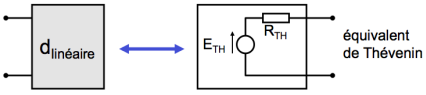
\includegraphics[scale=0.7]{img/image21.png}
	\captionof{figure}{Illustration du théorème de Thévenin}
\end{center}
Notons que $V_{th}$ est la tension à vide (ou fem à vide) entre les bornes du réseau (ici $d$ lorsque celui-ci est déconnecté de tout autre réseau. 
$Z_{th}$ est l'impédance, vue des bornes du réseau.


\subsubsection{Théorème et équivalent de Norton}
Le \textbf{théorème de Norton} est une variante du th. de Thévenin, utilisant cette fois une source de courant :\\
\prop{Tout réseau linéaire et permanent est équivalent à une source de \textit{courant} unique $I_N$ en \textit{parallèle} avec une impédance $Z_N$.}
\begin{center}
	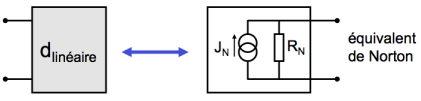
\includegraphics[scale=0.7]{img/image22.png}
	\captionof{figure}{Illustration du théorème de Norton}
\end{center}


Une multitude d'exemples d'applications sont disponibles dans les slides (24-31)\\
Les démonstrations de ces théorèmes sont à connaître (slide 31 et page 127-128).

\subsection{Impédance d'entrée, impédance de sortie}
\subsubsection{Équivalent de Thévenin d'un dipôle charge : résistance d'entrée}
Supposons qu'un appareil (une charge) doivent recevoir une tension à ses bornes. S'il est linéaire, il lui correspond un équivalent de Thévenin possédant le même comportement électrique.\\

Pour se faire, on définit la \textbf{résistance d'entrée} $R_{in}$ d'un dipôle charge linéaire comme la valeur de la résistance équivalente (au sens de Thévenin) à ce dipôle. Autrement dit :
\begin{itemize}
	\item La valeur de la résistance de l'équivalent de Thévenin du dipôle
	\item L'inverse de la pente de la caractéristique de ce dipôle
	\item La résistance par laquelle on peut remplacer ce dipôle sans modifier le fonctionnement du circuit extérieur
\end{itemize}\ \\
\prop{La résistance d'entrée est avant tout un \textit{nombre} caractérisant le comportement externe du dipôle ([$\Omega$])}\ \\
Ce n'est donc \textbf{PAS} (sauf exception rare) la résistance qui se trouve à l'entrée du circuit !
\subsubsection{Interprétation}
Si un dipôle possède une résistance d'entrée de $500\Omega$ cela signifie simplement que si on lui applique une tension de $10V$ il consommera comme courant $20 mA$.\\

Cette notion permet de remplacer, du point de vue du circuit extérieur, un montage complexe par une résistance fictive unique.

\subsubsection{Équivalent de Thévenin d'un dipôle source : résistance de sortie et fem à vide}
Pour autant que le circuit soit linéaire, il peut être modélisé par un circuit équivalent de Thévenin. Définissons :
\begin{description}
	\item[Résistance de sortie] ; Valeur de la résistance de l'équivalent de Thévenin de ce dipôle.
	\item[Fem à vide] ; Valeur de la source de tension idéale de l'équivalent de Thévenin de ce dipôle.
\end{description}

\subsubsection{Interprétation}
\begin{wrapfigure}[8]{r}{3cm}
	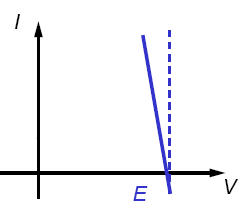
\includegraphics[scale=0.4]{img/image20.png}
	\captionof{figure}{Influence de la résistance de sortie}
\end{wrapfigure}
La \textit{fem à vide} est la valeur de la tension visible à la sortie du dipôle lorsque celui-ci ne délivre aucun courant. La tension à la sortie du dipôle valant (dans ce cas $I = 0A$) :
\begin{equation}
	V = e_{out} - R_{out}I
\end{equation}
Cette équation permet également de comprendre la \textit{résistance de sortie}. Lorsqu'un courant passe, la résistance de sortie introduit une certaine chute de tension. La tension de sortie est donc plus basse que la fem à vide.\\

\prop{La résistance de sortie traduit la difficulté du dipôle à maintenir sa tension de sortie constante lorsque le courant délivré augmente.}


\setcounter{subsection}{3}
\subsubsection{Équivalent de Thévenin/Norton d'un quadripôle}
\begin{wrapfigure}[8]{l}{4.7cm}
	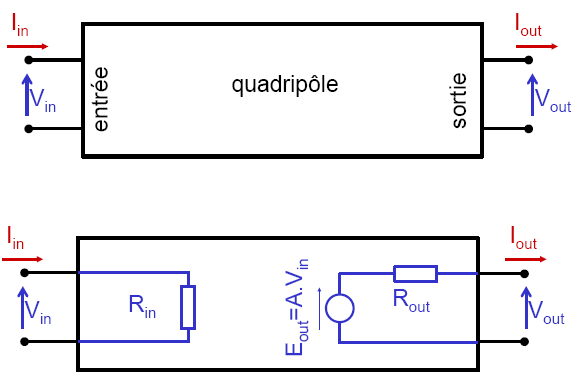
\includegraphics[scale=0.3]{img/image23.png}
	\captionof{figure}{Equivalent de Thévenin d'un quadripôle}
\end{wrapfigure}
Il suffit de modéliser l'entrée et la sortie par un équivalent de Thévenin comme précédemment. L'appareil sera caractérisé lors de la connaissances de trois paramètres :
\begin{enumerate}
	\item Sa résistance d'entrée $R_{in}$
	\item Sa résistance de sortie $R_{out}$
	\item Sa fem à vide ($e_{out}$)
\end{enumerate}
Il existe bien entendu cette fois une tension d'entrée, de sortie et même chose pour le courant.


\subsection{Adaptation d'impédance}
\subsubsection{Connecter deux appareils : pas si simple !}
Soit le cas ou on souhaite connecter un apareil en "amont" (source délivrant un signal) à un appareil en "aval" (charge recevant ce signal)\footnote{Chacun de ces appareils sont typiquement des quadripôles.}. Un principe de base est à retenir :\\
\prop{On \textbf{ne} peut \textbf{pas} interconnecter des composants et des montages sans effectuer certaines \textit{vérification}.}\ \\

Il faut :
\begin{enumerate}
	\item Vérifier que l'appareil en aval supporte les niveaux de tensions délivrés par l'appareil en amont (risque de dommages)
	\item Vérifier l'\textbf{adaptation d'impédance}, c'est-à-dire que les résistance d'entrée et de sortie sont "compatibles".\footnote{On pourrait sinon "bloquer" une grande partie du signal.} Ces critères diffèrent suivant que l'on veut transmettre une tension, un courant ou une puissance.
\end{enumerate}

\subsubsection{Adaptation d'impédance en tension}
Si l'on connecte deux appareil (modélisés par leur équivalent de Thévenin), on modifie la tension présente à l'entrée de l'appareil en aval (gauche) qui ne vaut plus $E$ : formule du diviseur résistif :
\begin{equation}
	\left\{\begin{array}{l}
	I = \frac{E}{R_{in} + R_{out}}\\
	V = R_{in} I
	\end{array}\right.
\end{equation}
et donc : 
\begin{equation}
	V = \frac{R_{in}}{R_{in} + R_{out}}E
\end{equation}
\begin{wrapfigure}[5]{l}{5.5cm}
	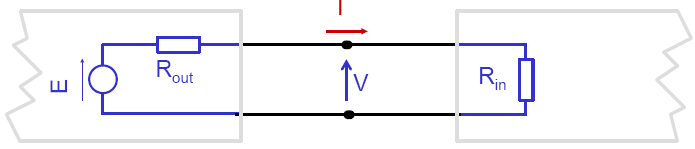
\includegraphics[scale=0.3]{img/image24.png}
	\captionof{figure}{Adaptation d'impédance en tension}
\end{wrapfigure}
Le signal de l'appareil en amont est affaibli. Pour éviter toute dégradation, ce "rapport de résistance" doit être proche de l'unité. Le \textbf{critère d'adaptation d'impédance en tension} est donc :\\
\prop{Lorsqu'on désire transmettre un signal de tension, l'impédance de sortie doit être faible devant l'impédance d'entrée.}


\subsubsection{Adaptation d'impédance en courant}
Reprenons le cas de figure précédent si ce n'est que l'appareil en amont se comporte comme une \textbf{source de courant}. La sortie de l'appareil en amont est décrite par un équivalent de \textit{Norton}. Calculons le courant reçu  par l'appareil en aval :
\begin{equation}
	\left\{\begin{array}{l}
	V = R_{in}\\
	V = R_{out}(J-I)
	\end{array}\right.
\end{equation}
\begin{wrapfigure}[6]{r}{4.7cm}
	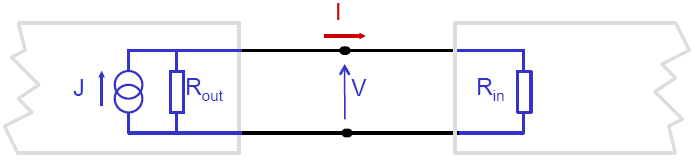
\includegraphics[scale=0.3]{img/image25.png}
	\captionof{figure}{Adaptation d'impédance en courant}
\end{wrapfigure}
Le courant dans l'appareil en avant vaut dès lors :

Le signal de l'app
\begin{equation}
	I = \frac{R_{out}}{R_{in} + R_{out}}J
\end{equation}
Cette fois, on trouvera une atténuation aussi faible que possible en suivant le \textbf{critère d'adaptation d'impédance en courant} :\\

\prop{Lorsqu'on désire transmettre un signal de courant, l'impédance d'entrée doit être faible devant l'impédance de sortie.}

\subsubsection{Adaptation d'impédance en puissance}
Prenons le cas général ou l'impédance d'entrée $Z_L$ est raccordée à une source de fem vide \underline{$E_S$} et d'impédance interne $Z_S$.\\
Le but est d'optimiser $Z_L$ ($Z_S$ étant supposé fixe) de façon à maximiser la puissance moyenne qu'elle absorbe, en régime sinusoïdal permanent.\\
La démonstration page 144 - 145 du syllabus nous donne le critère tant recherché...\\

\prop{Pour maximiser la puissance transmise de la source à la charge, l'impédance de charge doit être le complexe conjugé de l'impédance de source. \begin{equation}
	Z_L = Z^*_S
	\end{equation}}


\subsection{Cas particulier des appareils de mesure}
\subsubsection{Connexion d'un appareil de mesure}
Connecter un \textit{voltmètre} ou un \textit{ampèremètre} dans un circuit, cela revient à le modifier ! Analysons ceci grâce aux sections précédentes.\\
\begin{center}
	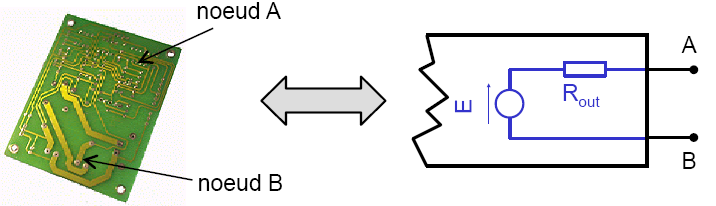
\includegraphics[scale=0.3]{img/image26.png}
	\captionof{figure}{Application de l'équivalent de Thévenin}
\end{center}
\textit{Remarque :} Les nœuds choisi pour mesurer une tension (par ex.) ne sont pas forcément des bornes d'entrée/sortie du montage. C'est la encore que l'équivalent de Thévenin va s'appliquer.

\subsubsection{Nœuds à haute et basse impédance}
\subsubsection{Impédance d'un nœud}
\begin{wrapfigure}[6]{r}{3.5cm}
	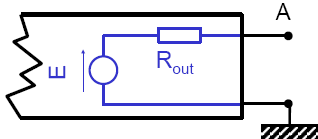
\includegraphics[scale=0.3]{img/image27.png}
	\captionof{figure}{Impédance de nœuds}
\end{wrapfigure}
Si l'un des deux nœuds est la masse, le montage est dit \textit{référencé à la masse} (B).\\
L'\textbf{impédance du nœud A} est la résistance de sortie de l'équivalent de Thévenin du montage.\\
On parle de noeud à \textit{haute} ou \textit{basse} impédance suivant la valeur de cette résistance de sortie (typiquement autour de $100 k\Omega$).


\subsubsection{Connexion d'un voltmètre}
\begin{wrapfigure}[6]{l}{4.7cm}
	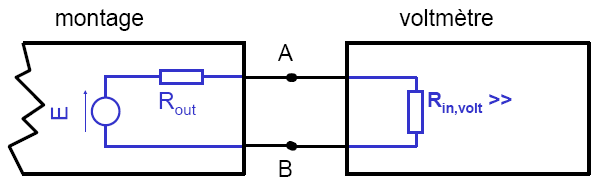
\includegraphics[scale=0.3]{img/image28.png}
	\captionof{figure}{Cas du voltmètre}
\end{wrapfigure}
On saura que l'on ne perturbe pas le montage en branchant un voltmètre suivant le critère d'adaptation d 'impédance en tension. Le voltmètre doit avoir \textit{une impédance d'entrée beaucoup plus élevée que l'impédance existant entre les nœuds utilisés pour faire la mesure.}\ \\

\subsubsection{Connexion d'un ampèremètre}
\begin{wrapfigure}[6]{r}{4cm}
	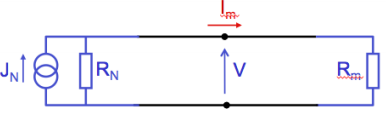
\includegraphics[scale=0.3]{img/image29.png}
	\captionof{figure}{Cas de l'ampèremètre}
\end{wrapfigure}
Un  ampèremètre se connecte en \textit{série} pour mesurer un courant, il faut donc obligatoirement interrompre un fil de ce circuit. Il faudra cette fois utiliser un équivalent de Norton. Des résultats précédents, on peut conclure que l'\textit{impédance d'entrée de l'ampèremètre doit être beaucoup plus faible que l'impédance existant entre les nœuds entre lesquels on insère l'ampèremètre}\footnote{Le but est bien d'essayer d'avoir la résistance la plus faible pour se comporter "comme un fil". \textit{Cf. Physique générale - Labo 1}}.





Les composants réactifs ne consomment ou ne génèrent pas de puissance, mais peuvent en stocker momentanément et la restituer ensuite : implique que le \textit{temps} doit être pris en compte.




\newpage
\section{Composants réactifs et outils associés}
\subsection{Analyse temporelle du circuit RC}
\subsubsection{Résolution analytique complète}
Voir syllabus page 201-204.
\begin{center}
	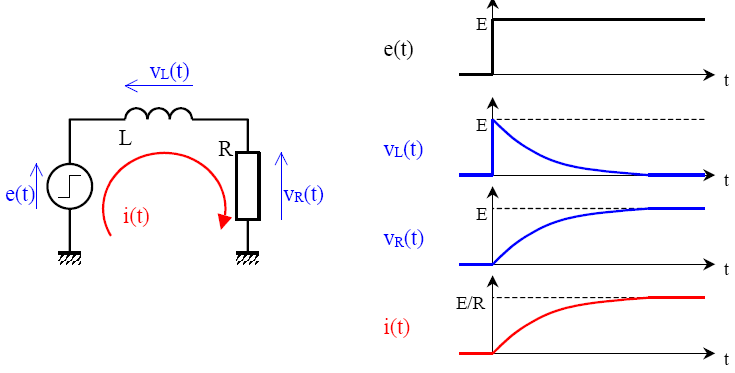
\includegraphics[scale=0.4]{img/image11.png}
	\captionof{figure}{Résolution circuit RC}
\end{center}

\subsubsection{Résolution rapide}
\subsubsection{Avant l'échelon (condition initiale)}
\begin{enumerate}
	\item Le courant est nul vu la loi à long terme
	\item La ddp est constante et supposée nulle (1)
	\item La ddp sur la résistance est nulle (2)
\end{enumerate}
\begin{equation}
	\left\{\begin{array}{l}
	i(t_0^-) = 0\\
	v_C(t_0^-) = 0\\
	v_R(t_0^-) = 0
	\end{array}\right.
\end{equation}

\subsubsection{En t$_0$ (court terme)}
Que ce passe-t-il lorsque l'on applique l'échelon de tension $E$ ?
\begin{enumerate}
	\item La ddp de la capa reste nulle (ne peut varier instantanément)
	\item En conséquence de (1), toute la tension se reporte sur $v_R$
	\item Le courant est donné par Ohm
\end{enumerate}
\begin{equation}
	\left\{\begin{array}{l}
	v_C(t_0^+) = v_C(t_0^-) = 0\\
	v_R(t_0^+) = E\\
	i(t_0^+) = E/R
	\end{array}\right.
\end{equation}

\subsubsection{En $t = \infty$ (long terme)}
\begin{enumerate}
	\item Le courant est nul dans la capacité (loi long terme)
	\item En conséquence de (1) la ddp sur la résistance est nulle
	\item Toute la tension est reportée sur la capa : $v_C = E$.
\end{enumerate}

\subsubsection{Résolution rapide (2e exemple) : échelon des tension inverse}
En partant de la situation finale du cas précédent, voyons ce qui se passe en appliquant une tension négative d'amplitude E. On suppose que l'instant $t=0$ représente le moment de retour à 0 de la tension $e(t)$.

\subsubsection{Avant l'échelon (conditions initiales)}
\begin{enumerate}
	\item Le curant et la ddp sur la résistance sont nuls
	\item La ddp sur la capa vaut E (capa chargée)
\end{enumerate}

\subsubsection{En $t_0$ (court terme)}
Juste après l'échelon négatif $-E$
\begin{enumerate}
	\item La source de tension prend la valeur nulle ! $e(t_0^+) = 0$
	\item La ddp de la capa ne peut pas varier directement : elle vaut encore $+E$
	\item En conséquence, la tension de la résistance vaut $-E$
	\item Le courant vaut donc $-E/R$
\end{enumerate}

\subsubsection{En $t = \infty$ (long terme)}
\begin{enumerate}
	\item Le courant est nul dans la capacité (loi long terme)
	\item La tension est nulle dans la résistance à cause de (1)
	\item comme $v_R$ et $e(t)$ sont nulles, $v_C$ l'est aussi (capacité complètement déchargée)
\end{enumerate}
\begin{center}
	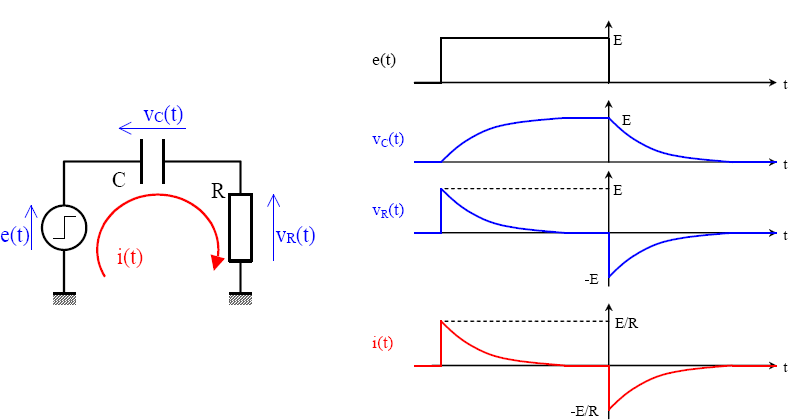
\includegraphics[scale=0.4]{img/image12.png}
	\captionof{figure}{Résolution circuit RLC en tension inverse}
\end{center}

\subsubsection{Constante de temps et fréquence de coupure (circuit du 1er ordre)}
La durée de la charge et décharge de la capacité dépend de la constante de charge : $\tau = RC$.
\begin{center}
	\begin{tabular}{|c|c|}
		\hline 
		Temps écoulé depuis l'échelon & Pourcentage de la (dé)charge réalisé \\ 
		\hline 
		$\tau$                           & 63                                      \\ 
		\hline 
		$3\tau$                          & 95                                      \\ 
		\hline 
		$5\tau$                          & 99                                      \\ 
		\hline 
	\end{tabular} 
\end{center}
On dira également que
\begin{itemize}
	\item $v_C(t)$ est un filtre passe-bas de $e(t)$
	\item $v_R(t)$ est un filtre passe-haut de $e(t)$
\end{itemize}
La limite entre les fréquences hautes et basses est donnée par la fréquence de coupure définie par
\begin{equation}
	f_0 = \frac{1}{2\pi\tau}
\end{equation}
\subsection{Analyse temporelle du circuit RL}
\subsubsection{Résolution analytique complète}
Si l'on attend suffisamment longtemps, par la loi \textit{long terme} $V = 0$ sur la self et $I = cste$ (pas forcément nul).\\
On peut résoudre ce circuit analytiquement (syllabus page 212, slide 54- 57)

\subsubsection{Résolution rapide}
Même raisonnement que pour le circuit RC (page 212 pour le RL)

\subsubsection{Constante de temps et fréquence de coupure}
Les résultats ci-dessus nous apprennent que
\begin{itemize}
	\item La tension $v_L(t)$ ne comporte que les hautes fréquences du signal $e(t)$ : filtre passe-haut
	\item La tension $v_R(t)$ ne comporte que les basses fréquences
\end{itemize}
 


\subsection{Analyse temporelle du circuit RL (source sinusoïdale)}
Au lieu d'avoir $e(t) = cste$, on a $e(t) = V_m\cos(\omega t + \alpha)$
\begin{equation}
	Ri + L\frac{di}{dt} = e(t)
\end{equation}
Il suffit après de résoudre l'équation différentielle comme au cours d'Analyse I.

\subsection{Circuit RLC avec précharge}
La capacité à été préalablement chargée avec une tension $v_0$ et à l'instant $t=0$ on ferme l'interrupteur. L'équation du circuit est donc :
\begin{equation}
	v_0 - \frac{1}{C}\int_{t_0}^t i(t)dt = L\frac{di}{dt} + Ri(t)
\end{equation}


\subsection{Fonctions de transfert}
\subsubsection{Plan de Bode}
La fonction de transfert $H(j\omega)$ est le rapport des phraseurs d'entrée et de sortie. C'est l'"opération" réalisée par le circuit. Elle se présente généralement :
\begin{equation}
	H(j\omega) = A(\omega)e^{j\phi(\omega)}
\end{equation}
où $A(\omega)$ est l'amplitude et $\phi(\omega)$ la phase\footnote{Attention, $H(j\omega)$ n'est \textbf{pas} un phaseur !}.\\

Les fonctions de transferts sont représentées dans le \textit{plan de Bode} :
\begin{description}
	\item[Gain] : Graphique bilogarithmique (log[$A(\omega)$] = f(log($\omega$))
	\item[Phase]: Graphique semi-logarithmique ($\phi(\omega)$ = f(log($\omega$))
\end{description}

\subsubsection{Décibels}
C'est une unité adimensionelle pour exprimer un rapport, comme par exemple le rapport de tension ou de courant :
\begin{equation}
	X[dB] = 20\log(X)
\end{equation}

Plus utile encore, le rapport de puissances :
\begin{equation}
	X[dB] = 10\log(X)
\end{equation}
Son intérêt se trouve dans le fait que les équipement électroniques sont composés de modules successifs, il suffira dès lors d'additionner des décibels de chaque module.